\documentclass[conference]{IEEEtran}

\usepackage[sort&compress]{natbib}

% *** GRAPHICS RELATED PACKAGES ***
\usepackage[dvips]{graphicx}
\usepackage{balance}
% *** MATH PACKAGES ***
\usepackage{amsmath}
\usepackage{pgfplots}
\usepackage{amssymb}
\usepackage{booktabs}
% *** SPECIALIZED LIST PACKAGES ***
%
\usepackage{algorithmic}
% *** ALIGNMENT PACKAGES ***
%

\usepackage[caption=true]{caption}
\usepackage{epstopdf}
\usepackage{multicol, blindtext}
\usepackage{url}


\usepackage{amsmath,amsthm,amssymb,epsfig} %cong thuc toan
\usepackage{etex}
\usepackage{array} % cho table
\usepackage{multirow} % gop dong table
\usepackage{subcaption}
\usepackage[colorlinks]{hyperref}
\newcolumntype{P}[1]{>{\centering\arraybackslash}p{#1}}
\newcolumntype{M}[1]{>{\centering\arraybackslash}m{#1}}

\DeclareMathOperator*{\argmin}{argmin}

\begin{document}
%
% paper title
% Titles are generally capitalized except for words such as a, an, and, as,
% at, but, by, for, in, nor, of, on, or, the, to and up, which are usually
% not capitalized unless they are the first or last word of the title.
% Linebreaks \\ can be used within to get better formatting as desired.
% Do not put math or special symbols in the title.
\title{Fully Residual Neural Networks for Aerial Image Segmentation}

\author{\IEEEauthorblockN{Dinh Viet Sang}
\IEEEauthorblockA{Hanoi University of Science\\ and Technology\\
Email: sangdv@soict.hust.edu.vn}\\
\and
\IEEEauthorblockN{Nguyen Duc Minh}
\IEEEauthorblockA{FPT Technology Research Institute\\
FPT University \\
Email: minhnd33@fpt.com.vn}\\
}


% make the title area
\maketitle


\begin{abstract}
Semantic segmentation from aerial imagery is one of the most essential tasks in
the field of remote sensing with various potential applications ranging from map
creation to intelligence service.
One of the most challenging factor of these tasks is the very heterogeneous
appearance of artificial objects like buildings, cars and natural entities such
as trees, low vegetation in very high-resolution digital images. In this paper,
we propose a very deep feature learning approach with fully convolutional
networks (FCN) for semantic segmentation. Particularly, we introduce one more
skip connection while upsampling the feature maps in FCN architecture using the
famous ResNet101 encoding network. The benchmark results from ISPRS 
which our proposed method attains much better accuracies in comparison with
other recent state-of-the-art methods on the well-known Vaihingen and Potsdam
datasets from ISPRS Working Group II/2.

\end{abstract}

%\IEEEpeerreviewmaketitle

\section{Introduction}
In the last 20 years, a huge amount of effort has been spent on solving semantic
segmentation problem in aerial photography. However, the task is still
considered not being solved yet. Many advanced machine learning techniques have
been applied to train and learn efficient models and many promising results have
been made in the 2D Semantic Labeling Contest. Furthermore, with the rise of
generally available computational resources, a large number of deep learning
models which can learn so much useful insight and pattern from raw data without
providing the models with much human domain knowledge to produce even better
results.

Semantic segmentation in aerial images is a key task in remote sensing with many
applications. For instance, data acquired by airborne sensors can be applied to
urban planning to identify different urban areas such as vegetation, buildings,
transportation infrastructure or even traffic flow to help design and develop
a town or city with a long-term vision. However, to accurately attain a
correctly segmented images from raw data from aerial cameras is a very severe
and painful task which requires so much domain knowledge in both remote sensing
and computer science. To our knowledge, no fully automated methods have been
devised to solve this very core problem yet because different data from
different regions for different tasks needs different approaches. Since 2014, a
2D semantic labelling contest has been held by ISPRS WG III/4 is meant to
resolve is issue. The first place of this competition
\cite{segmentationcompetition} to date on both Vaihingen and Potsdam datasets
is HUSTW team with 91.6\% overall accuracy on the hidden test set.

In this paper, we propose a powerful deep learning approach which can unleash
the segmentation potential of ResNet which has won the 1st place on the ILSVRC
2015 classification task. Particularly, we combine ResNet101 with FCN for
solving the semantic segmentation task. Moreover, we experiment two different
FCN architectures with 2 and 3 skip connections and both of them demonstrate
the same overall accuracy on Vaihingen dataset and achieve the 4th position
globally with 91\% accuracy on the hidden test set by ISPRS. Similarly, our
3-skip model also obtain 91.1\% accuracy on the hidden test set from Potsdam
dataset with the 3rd position globally.

The rest of the paper is organized as follows. In section 2, we review related
work in deep learning and semantic segmentation. In section 3, we briefly
introduce our proposed approach. Finally, in section 4, we show the experimental
results on both Vaihingen and Potsdam dataset and compare our approach with
recent state-of-the-art methods.

\section{Related work}
Classical approaches for semantic segmentation from aerial images are often
based on many extracted features and building typical classification models
such as random forest and conditional random field. Despite the fact that
these and combination of the two can perform with such a small amount of time,
but many deep learning models can achieve better overall accuracies.

In recent years, deep learning has proved its potential in many field,
especially in computer vision. These neural network based models can learn
much of the hand-engineering features automatically as long as provided with
enough good labelled data. The first known convolutional neural network is
LeNet used to solve the classification task of ten handwritten digits from 0 to
9. However, until 2012, AlextNet came to public with the winner of ImageNet
ILSVRC challenge. Since then, many typical recognition CNNs has been proposed
and performed impressively in one of the most pretigious computer vision
competitions - the annual ImageNet Large Scale Visual Recognition Challenge
(ILSVRC). These nets tend to be both wider and deeper with the heavy use of
batch normalisation after every weight layer to improve the optimization ability
and curb overfitting problem of these deep learning models.

Those classification networks are not only used in classification tasks. Each
of them can also act as an image encoder. In \cite{long2015fully}, Long propose
a new semantic segmentation architecture, which is called fully convolutional
neural network (FCN). To encode a raw image as the input data, the FCN encodes
the raw image into a set of feature maps which retain only semantic information
about objects and textures of the input image using any visual recognition
network without any fully-connected layers among it.

In 2D semantic labelling contest on ISPRS, the top teams use many variations of
fully conditional networks that set the state-of-the-are on both Vaihingen and
Potsdam datasets. In \cite{duydensenet} and \cite{duyvgg19}, the author
successfully apply a FCN using VGG19 to 2D semantic segmentation problem and
achieve better overall accuracy than previous methods.

\section{Our proposed approach}
\subsection{Deep residual network}

Deep residual networks (ResNets) \cite{he2016deep} achieved
1st-place winning entries in all five main tracks of the ImageNet and COCO 2015
competitions, which covered image classification, object detection and semantic
segmentation. ResNet architectures are much deeper than the preceeded ones which
are VGG architectures (with both 16 and 19 weight layers). With the heavy use of
batch normalization and the introduction of residual blocks periodically stacked
throughout the network.

A typical ResNet consists of multiple \textit{residual blocks} and heavy
application of \textit{batch normalization} between every convolutional layer
and ReLU layer.

\begin{center}
	\begin{figure*}
		\begin{center}
			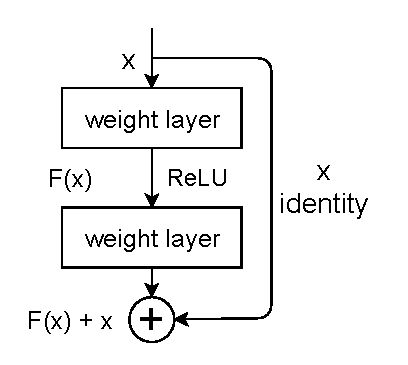
\includegraphics[scale=1]{image/Skip_ResNet}
		\end{center}
		\caption{A residual block - the fundamental building block of residual
		networks \cite{he2016deep}.}
		\label{residualblock}
	\end{figure*}
\end{center}

\begin{center}
	\begin{figure*}
		\begin{center}
			\includegraphics[scale=.25]{image/FCN-ResNet}
		\end{center}
		\caption{FCN-ResNet.}
		\label{fcn-resnet}
	\end{figure*}
\end{center}

\begin{center}
	\begin{figure*}
		\begin{center}
			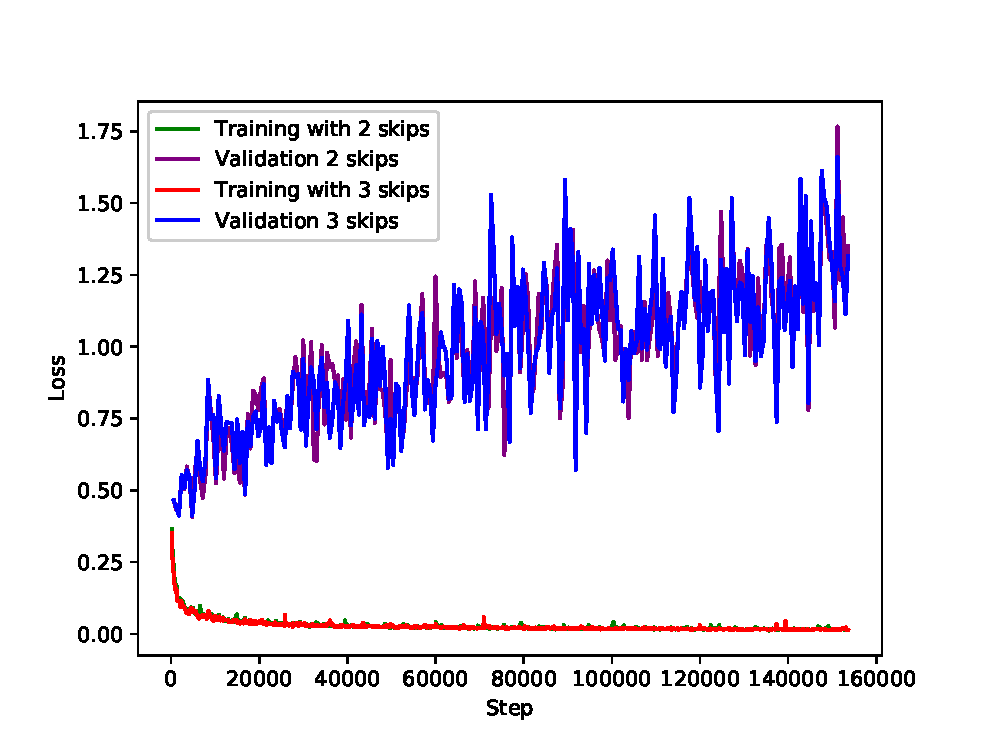
\includegraphics[scale=.75]{image/4losses}
		\end{center}
		\caption{Losses of 4s and 8s.}
		\label{4s_8s_losses}
	\end{figure*}
\end{center}

\begin{center}
	\begin{figure*}
		\begin{center}
			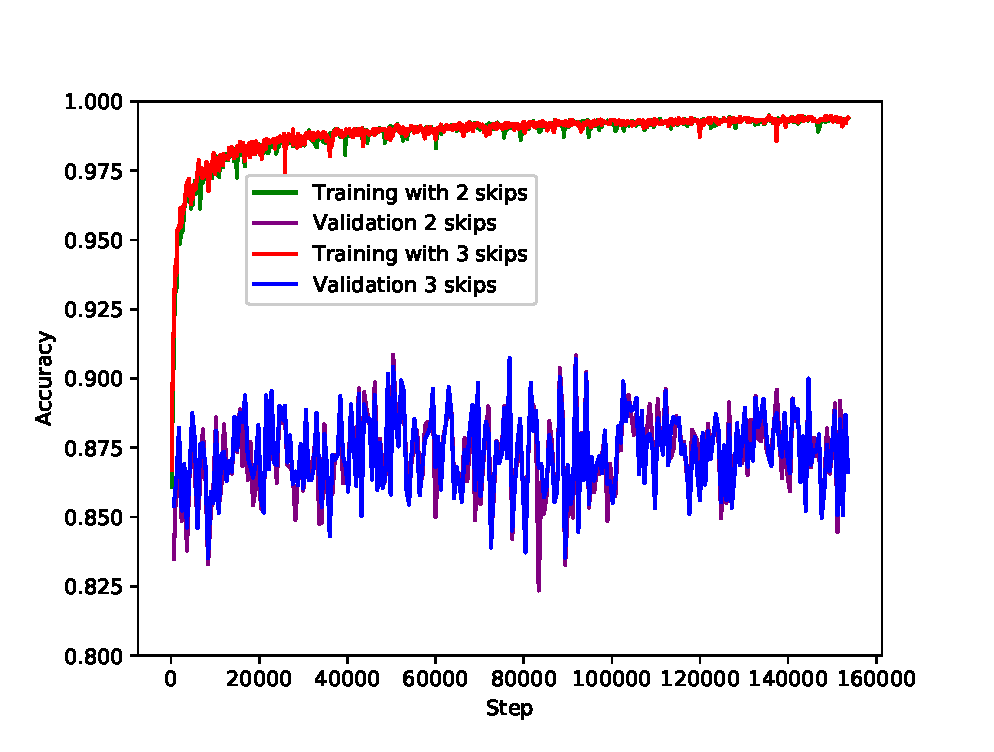
\includegraphics[scale=.75]{image/4accs}
		\end{center}
		\caption{Accuracies of 4s and 8s.}
		\label{4s_8s_accs}
	\end{figure*}
\end{center}

\begin{center}
	\begin{figure*}
		\begin{center}
			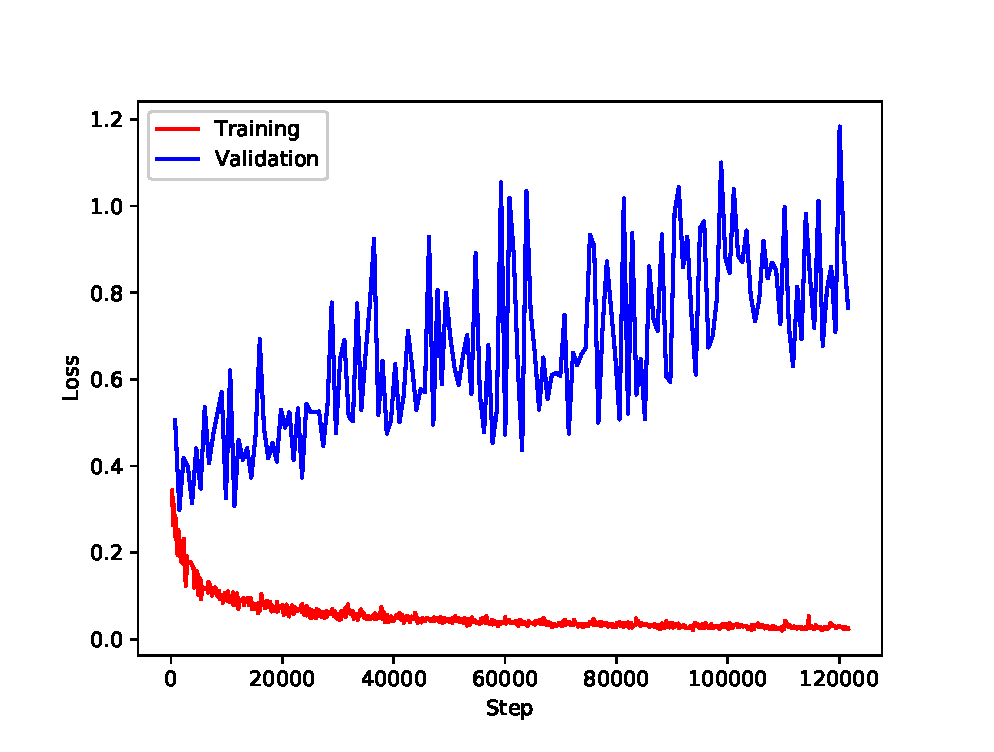
\includegraphics[scale=0.75]{image/FCN-4s-ResNet101_Potsdam_loss}
		\end{center}
		\caption{FCN-4s-ResNet101\_Potsdam\_loss.}
		\label{residualblock}
	\end{figure*}
\end{center}

\begin{center}
	\begin{figure*}
		\begin{center}
			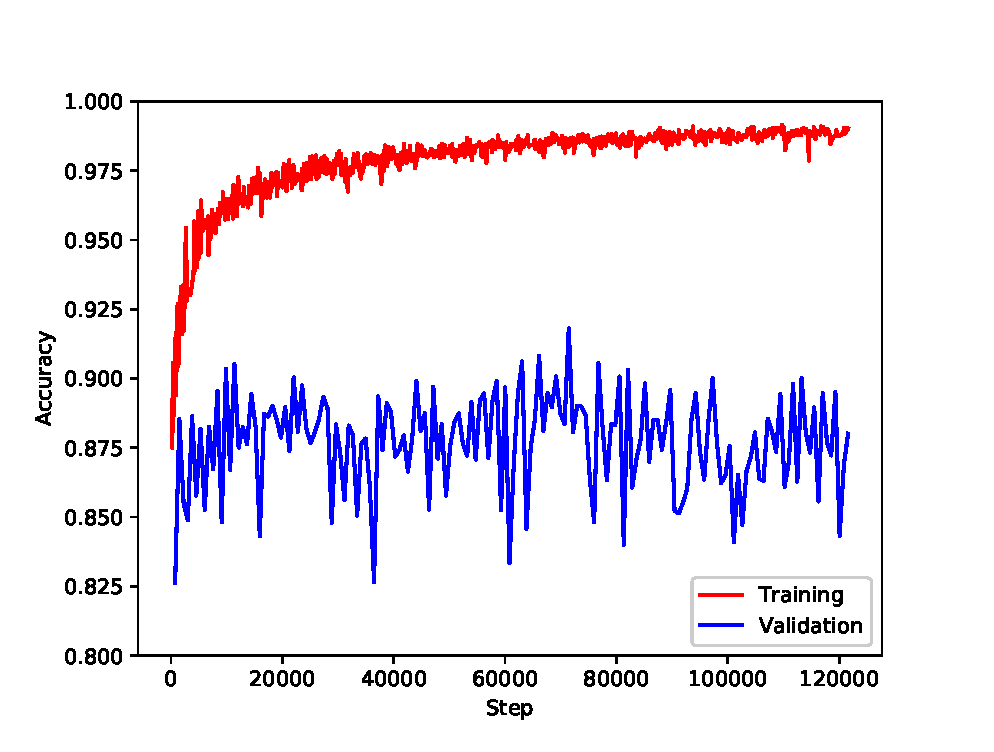
\includegraphics[scale=0.75]{image/FCN-4s-ResNet101_Potsdam_acc}
		\end{center}
		\caption{FCN-4s-ResNet101\_Potsdam\_acc.}
		\label{residualblock}
	\end{figure*}
\end{center}

\textbf{Residual blocks:} Instead of directly approximate $H(x)$ underlying
mapping by stacking a few more intermediate layers, another mapping of
$F(x) = H(x) - x$ is fit  by the stacked nonlinear layers. The original
function is now recast into $F(x) + x$. Therefore, it is easier to optimize
the residual mapping than to optimize the original.

%\begin{center}
%	\begin{figure*}
%		\begin{center}
%			\includegraphics[scale=.4]{image/composite.eps}
%		\end{center}
%		\caption{Composite function with bottleneck layer \cite{huang2017densely}.}
%		\label{composite}
%	\end{figure*}
%\end{center}

The fundamental building block of ResNet architectures in
Fig.~\ref{residualblock} has been reformulated under the assumption that the
optimal function a block is trying to model is closer to an identity mapping
than to a zero mapping, and that it should be easier to find the perturbations
with reference to an identity mapping than to a zero mapping. This simplifies
the optimization of the network at almost no cost. Subsequent blocks in the
model are thus responsible for fine-tuning the output of a previous block,
instead of having to generate the desired output from scratch.

\textbf{Batch normalization:} 

Batch normalization draws its strength from making normalization a part of the
model architecture and performing the normalization for each training
mini-batch. Batch Normalization allows us to use much higher learning rates and
be less careful about initialization. It also acts as a regularizer, in some
cases eliminating the need for Dropout.

Batch normalization is similar to Dropout in the sense that it multiplies each
hidden unit by a random value at each step of training. In this case, the random
value is the standard deviation of all the hidden units in the mini-batch.
Because different examples are randomly chosen for inclusion in the
mini-batch at each step, the standard deviation randomly fluctuates. Batch
normalization also subtracts a random value (the mean of the mini-batch) from
each hidden unit at each step.

Both of these sources of noise mean that every layer has to learn to be robust
to a lot of variation in its input, just like with Dropout.

\subsection{Fully convolutional network}
Fully convolutional networks (FCN) popularized CNN architectures for dense
predictions without any fully-connected layers. This allowed segmentation maps
to be generated for image of any size and was also much faster compared to the
patch classification approach. Almost all the subsequent state-of-the-art
approaches on semantic segmentation adopted this paradigm.

A FCN architecture can be broadly thought of as an encoder network followed by
a decoder network:
\begin{itemize}
\item[-] The \textbf{encoder} is usually a pre-trained classification network
like VGG/ResNet followed by a decoder network;
\item[-] The task of the \textbf{decoder} is to semantically project the
discriminative features (lower resolution) learned by the encoder onto the pixel
space (higher resolution) to get a dense classification;
\end{itemize}

One issue in this specific FCN is that by propagating through several alternated
convolutional and pooling layers, the resolution of the output feature maps is
downsampled. Therefore, the direct predictions of FCN are typically in low
resolution, resulting in relatively fuzzy object boundaries.

\subsection{Cross-entropy loss}
Cross-entropy loss is widely used for training deep neural networks. Suppose
that $N$ is the number of pixels in the training data; $K$ is the number of
classes; $l_i$ is the correct class label of $i$-th sample; $\textbf{y}_i$ is
the one-hot encoding of the correct class label of $i$-th sample
($\textbf{y}_i(l_i) = 1$); and $\widehat{\textbf{y}}_i$ is the probability
distribution of $i$-th sample over classes. More importantly,
this semantic segmentation is mathematically a classification problem over
every pixel which each pixel is classified into $K$ classes. The
cross-entropy loss is defined as follows:
\begin{align}
L_S = -\dfrac{1}{N}\sum_{i=1}^{N}\sum_{j=1}^K\textbf{y}_i(j)
	log(\widehat{\textbf{y}}_i(j)),
\label{crossentropyal}
\end{align}
where $\textbf{y}_i(j) \in \{0,1\} $ indicates whether $j$ is the correct label
of $i$-th sample; $\widehat{\textbf{y}}_i(j) \in [0,1] $ expresses the
probability that $j$ is the correct label of $i$-th sample.

\subsection{Our Fully Convolutional Networks with ResNet101}
In this work, we propose 2 different FCN-ResNet101 architectures to deal with
the semantic segmentation problem on very high resolution data, namely
FCN-ResNet101-8s and FCN-ResNet101-4s. The encoder for both of them is a
pre-trained ResNet101 network on the ImageNet dataset for 1000-class
classification task. However, two different decoders are experimented for the
semantic segmentation task.

We first add a $1 \times 1$ convolution layer on top of \texttt{res5c\_relu}
layer to produce additional class predictions. Then we upsamples stride 2
predictions to get double-sized feature maps by performing transpose convolution
with the receptive field of $4 \times 4$. To combine predictions from both
upsampled volumes and the \texttt{res4b22\_relu} layer by implementing a skip
connection to fuse two of them which is just simply an addition operation. While
to build FCN-ResNet101-8s model just one more $2 \times$ upsampling and skip
connection are applied before the stride 8 predictions are upsampled back to the
image, FCN-ResNet101-4s model requires upto two more same $2 \times$ upsampling
and skip connection are applied before the stride 4 predictions are upsampled
back to the image. The receptive field of the stride 8 predictions and the
stride 4 predictions are $16 \times 16$ and $8 \times 8$.

For both models, we introduce Dropout to reduce the effect of overfitting by
applying only \texttt{res5c\_relu} layer due to very high channel dimension.

\section{Experiments and Evaluation}
\subsection{Datasets}
Vaihingen dataset and Potsdam dataset are provided on the 2D Semantic Labelling
Contest of ISPRS Working Group III/4 and both of them cover different urban
scenes in Germany. While Vaihingen is a quite small village with mostly detached
homes and multi-storey buildings, Potsdam shows a typical historic city with
large building blocks, narrow streets and dense settlement structures.

Labelled ground truth is provided for only one part of the data. The ground
truth of the remaining scenes will remain unreleased and stays with the
benchmark test organizers to be used for evaluation of submitted results.
While Vaihingen dataset contains 33 patches of different sizes and 16 of them
are provided with ground truth, Potsdam dataset consists of 38 patches which all
of them are of the same size and 24 of them are provided with ground truth,
$6000 \times 6000$. Each patch from both datasets consists of a true orthophoto
(TOP) extracted from a larger TOP mosaic.

We use 5-channel data when training on Vaihingen dataset (IR, R, G, nDSM and
DSM) and 6-channel data for Potsdam dataset (R, G, B, I, R, nDSM and DSM).
nDSM data from Potsdam dataset is generated by LAStools and supplied by ISPRS.

Each spatial position on the ground truth is labelled by one of six urban
objects: impervious surfaces, building, low vegetation, tree, car,
clutter/background (Fig.\ref{example_gt}).

\subsection{Data augmentation}
Due to very high resolution data and small number of patches in two datasets, we
use data augmentation techniques to generate more new data with out resizing
given images for the training phase. These techniques help us to reduce
information loss and, hence, to train a more robust network.

We used 3 main methods for data augmentation as follows: 
\begin{itemize}
\item[-] Randomly crop: Every TOP patch is randomly cropped for 4096 times with
the spatial dimension of $224 \times 244$ using uniform distribution;
\item[-] Entirely flip an image from left to right and upside down;
\end{itemize}
In practice, we find that applying augmentation techniques greatly improves the capacity of the model.

%\begin{figure}
%	\begin{tikzpicture}
%	\footnotesize
%	\begin{axis}[
%	width = 8.5cm,
%	symbolic x coords={Angry, Disgust, Fear, Happy, Sad, Surprise, Neutral},
%	xtick=data
%	]
%	\addplot[ybar,fill=blue] coordinates {
%		(Angry,   4953)
%		(Disgust,  547)
%		(Fear,   5121)
%		(Happy, 8989)
%		(Sad, 6077)
%		(Surprise, 4002)
%		(Neutral, 6198)
%	};
%	\end{axis}
%	\end{tikzpicture}
%	%\normalsize
%	\caption{Data distribution of FERC-2013.}
%	\label{dis}
%\end{figure}

%\begin{table*}
%	\caption{Overall Accuracy on the Vaihingen dataset}
%	\centering
%	\begin{tabular}{c|c|c}
%		\hline
%		\textbf{Method} & \textbf{Public test accuracy ( \%)} & \textbf{Private test accuracy (\%)}  \\
%		\hline
%		ResNet101 (team CASIA2 - rank 3 ISPRS) & $69.1$ & $91.1$ \\
%		FCN + F-CRF (team NLPR3 - rank 2 ISPRS) & $68.2$ & $91.2$ \\
%		U-net + DeconvNet (team HUSTW5 - rank 1 ISPRS) & 67.3 & $\textbf{91.6}$ \\
%		\hline
%		FCN-8s-VGG19 & $68.9$ & $89.8$\\
%		FCN-8s-VGG19 + ensemble & $69.1$ & $90.6$\\
%		DenseNet-BC & $69.5$ & $70.7$\\
%		DenseNet-BC + ensemble & $69.8$ & $71.0$\\
%		WideDenseNet & $70.1$ & $70.6$\\
%		WideDenseNet + ensemble & $70.2$ & $70.9$\\
%		WideDenseNet-BC & $70.2$ & $71.5$\\
%		WideDenseNet-BC + ensemble & $70.9$ & $71.9$\\
%		\hline
%		DenseNet + center loss & $69.0$ & $70.1$\\
%		DenseNet + ensemble + center loss & $69.4$ & $71.1$\\
%		DenseNet-BC + center loss& $68.9$ & $70.7$\\
%		DenseNet-BC + ensemble + center loss& $69.7$ & $70.9$\\
%		WideDenseNet + center loss& $70.2$ & $71.3$\\
%		WideDenseNet + ensemble + center loss& $\textbf{71.1}$ & $71.6$\\
%		WideDenseNet-BC + center loss& $70.6$ & $\textbf{72.2}$\\
%		WideDenseNet-BC + ensemble + center loss& $70.7$ & $\textbf{72.2}$\\
%		\hline
%	\end{tabular}
%	\label{compare}
%\end{table*}

\subsection{Implementation details}
Our experiments are conducted by using Python 3 with Tensorflow 1.4 framework on
a deep learning server with the following specifications: Intel Xeon CPU E5-2699
v4 88-core 2.20GHz Processor, Ubuntu Server 16.04.3 LTS 64-bit Operating System,
756GB of RAM and GPU NVIDIA GeForce GTX1080i with 11GB of GPU memory and compute
capability 6.1.

\textbf{Preparing dataset:} Since the images in both Vaihingen and Potsdam
dataset are cropped already, the preprocessing step is quite simple. Firstly,
we compute the mean image over the training set. Each pixel in the mean image
is computed from the average of all corresponding pixels (i.e. with the same
coordinates) across all training images. For each training image, we then
subtract from each pixel its mean value, and then set the standard deviation of
each pixel over all training images to 1.

\textbf{Optimization:} We train our models by Adam optimization algorithm with
the learning rate of $10^{-4}$ \cite{kingma2014adam}. We set the batch size
equal to 32 when training on Vaihingen dataset and 64 for Potsdam dataset.
Dropout is set at the rate of 50\%. All parameters in every batch normalization
layer are also retrained with Exponential Moving Average and decay 0.9.

\textbf{Fine-tuning phase:} All weights of two models are initialized with
pre-trained weight trained on ImageNet dataset including means, variances,
offsets, scales for batch normalization layers and also mean pixel values for
the first 3 input channels. Those which are additional layers such as the 2 or
3 last input layers (when using images with more than 3 channels), $1 \times 1$
convolution layer on top of \texttt{res5c\_relu} and filters for transpose
convolution are initialized randomly with a normal distribution which has mean
and standard deviation of zero and 0.02 respectively. Furthermore, mean pixel
value for DSM and nDSM are computed separately from pretrained weights, using
data from diven datasets. Finally, we fine-tune all layers by backpropagation
through the whole net.

\textbf{Testing phase:} In the testing phase, we ensemble different checkpoints
obtained during the training phases to increase the robustness and the power of
the learned classifier. In this paper, we simply keep the last fifteen
checkpoints corresponding to the last fifteen training epochs for inference.

\subsection{Experimental results}

 
\section{Conclusion}
In this paper, we propose an effective approach to ...

In the future, we would like to exploit ...

\balance
\bibliographystyle{abbrv}
\bibliography{references}

\end{document}
